\documentclass[11pt, a4paper]{article}

\usepackage{graphicx}
\usepackage[a4paper,top=3cm,bottom=2cm,left=2cm,right=2cm,marginparwidth=1.75cm]{geometry}
\usepackage[english]{babel}
\usepackage[utf8x]{inputenc}
\usepackage{subfig}
\usepackage{amsmath}
\usepackage{amssymb}
\usepackage{cancel}

\graphicspath{ {./images} }
\newcommand*{\qed}{\hfill\ensuremath{\quad\square}}%
\newcommand*{\rad}{\ensuremath{\,\text{rad}}}
\newcommand*{\R}{\ensuremath{\mathbb{R}}}

\makeatletter
\renewcommand*\env@matrix[1][*\c@MaxMatrixCols c]{%
  \hskip -\arraycolsep
  \let\@ifnextchar\new@ifnextchar
  \array{#1}}
\makeatother

\newtheorem{theorem}{Theorem}

%------------------------------------------------
%Templates for images and figures
% \begin{figure}[h]
%   \centering
%   \subfloat[caption 1]{{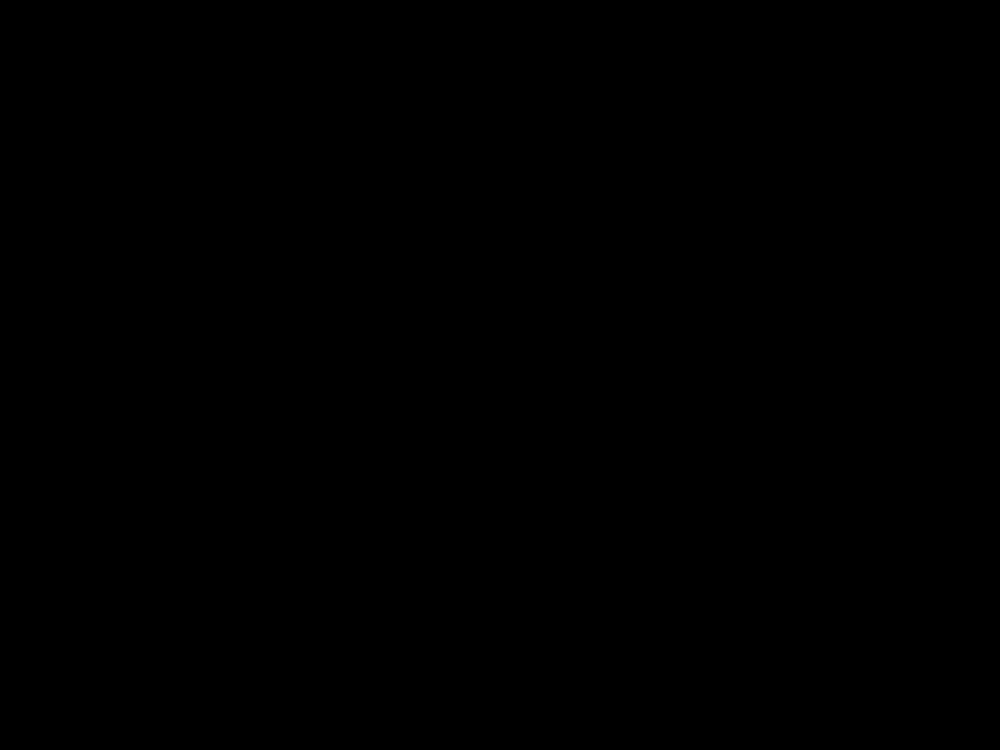
\includegraphics[width=30mm]{images/placeholder.png}}}%
%   \qquad
%   \subfloat[caption 2]{{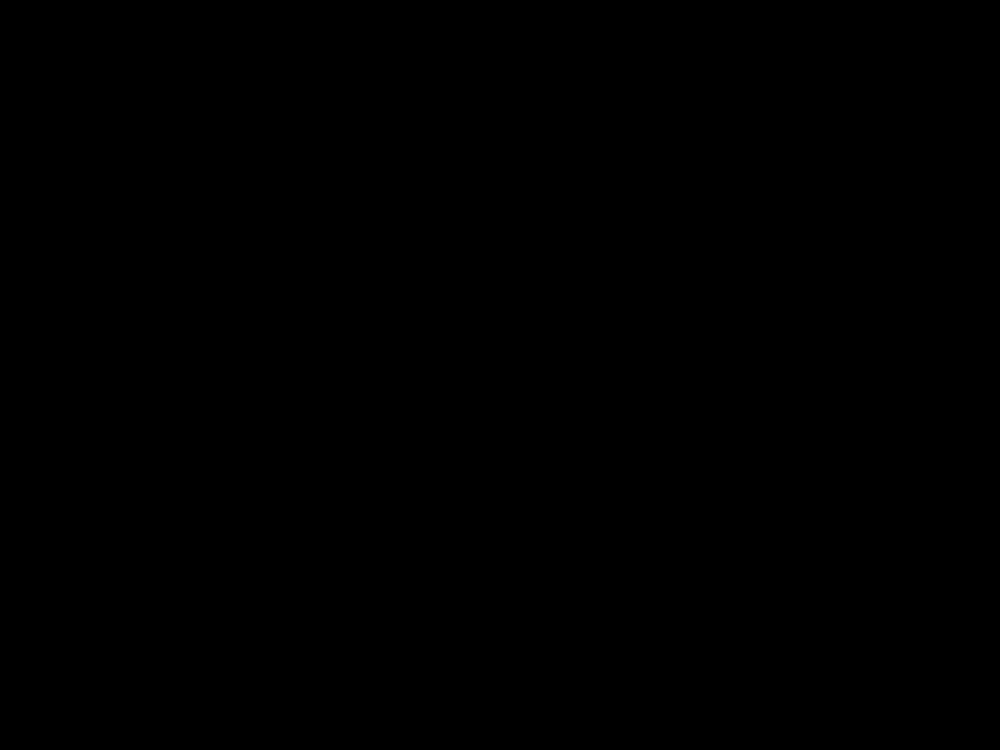
\includegraphics[width=30mm]{images/placeholder.png}}}%
%   \caption{Description}
% \end{figure}

% \begin{figure}[h]
%   \centerline{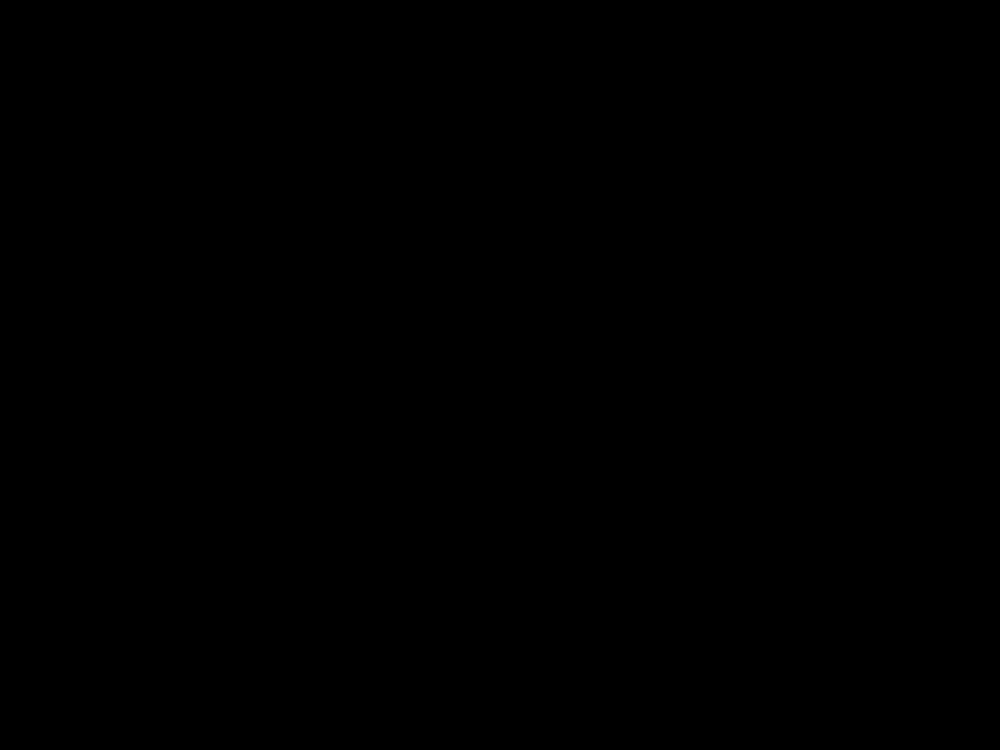
\includegraphics[width=50mm]{images/placeholder.png}}
%   \caption{Description}
% \end{figure}
%-----------------------------------------------

\begin{document}
\setcounter{equation}{0}
\setcounter{section}{4}

\section{Thermofluids Lecture 5: The ideal gas and equations of state}


\subsection{Equations of state for an ideal gas}
The intesive properties of $\{p, v, T \}$ are in fact not independent of one another. The relation between these properties is referred to as an equation of state. The equation of state for an ideal gas is given by the following relation:
\begin{equation}
  pV = n \bar{R}T \quad \text{or} \quad pv = RT
\end{equation}
Where $R$ is the specific gas constant given by the relation:
\begin{equation}
  R = \frac{\bar{R}}{M}
\end{equation}
It's important to know that assuming ideal gas is not always valid. To determine how close the behaviour of a gas is to the behaviour of an ideal gas we define a compressibility factor $Z$:
\begin{equation}
  Z = \frac{pv}{RT}
\end{equation}
The compressibility factor of an ideal gas is equal to $1$ by definition. In general $Z$ increases with pressure and decreases with temperature. The important take away here is that $Z$ starts to deviate from the ideal case more and more when aproaching the critical point or the boiling point.


\subsection{Notation and terminology}
The next section will deal with both total derrivatives and partial derrivatives so it's worth going over some notation very quickly:
\begin{equation}
  du(v, p) = \left( \frac{\partial u}{\partial v} \right)_p dv + \left( \frac{\partial u}{\partial p} \right)_v dp
\end{equation}
These lecture notes will use the letter $d$ for denoting the total derrivative with respect to some variable., $\partial$ for the partial derrivative and $\delta$ for an inexact differential. The small $p$ and $v$ to the right of the differentials denote that that variable stays constant when taking the derrivatives.\\
Some of the following terms will also be used:
\begin{itemize}
  \item \underline{isobar}, line along which pressure stays constant
  \item \underline{isotherm}, line along which temperature stays constant
  \item \underline{isochore}, line along which specific volume stays constant.
\end{itemize}


\subsection{specific heat capacity}
The specific heat at constant volume is given by the following relation:
\begin{equation}
  c_v = \left( \frac{\partial q}{\partial T} \right)_v
\end{equation}
Which is the rate of change of the specific heat $q$ with repsect to the temperature $T$ along an isochore. Recall the first law of thermodynamics in differential form:
\begin{align}
  du = &\delta q - \delta w\\
       &\delta q = du + \delta w = du + pdv \notag
\end{align}
When we subsitute this first law back into the equation of the specific heat at constant volume we get the following expression:
\begin{equation*}
  c_v = \left( \frac{\partial u}{\partial T} \right)_v + \cancelto{0}{\left( p \frac{\partial v}{\partial T} \right)_v}
\end{equation*}
Note that the second term cancels to zero because we are considering the rate of change at constant volume. The term $\partial v$ will thus also be constant. The rate of change of a constant is $0$ thus the entire term cancels to $0$. This leaves the following expression for the specific heat along an isochore:
\begin{equation}
  c_v = \left( \frac{\partial u}{\partial T} \right)_v
\end{equation}
\\
Now consider the same equation but at constant pressure rather then constant volume:
\begin{equation}
  c_p = \left( \frac{\partial q}{\partial T} \right)_p
\end{equation}
When applying the first law of thermodynamics again we get the follwing expression:
\begin{align*}
  c_p &= \left( \frac{\partial u}{\partial T} \right)_p + \left( p \frac{\partial v}{\partial T} \right)_p \\
      &= \left( \frac{\partial u}{\partial T} \right)_p + \left( \frac{\partial pv}{\partial T} \right)_p + \cancelto{0}{\left( v \frac{\partial p}{\partial T} \right)_p}
\end{align*}
This leaves us with:
\begin{equation}
  c_p = \left( \frac{\partial(u + pv)}{\partial T} \right)_p
\end{equation}
The term $u+pv$ is something very important in thermodynamics. Because of this we define a new variable referred to as enthalpy denoted by $h$ and $H$ for specific enthalpy and total enthalpy respectivly. This gives us:
\begin{equation}
  h = u + pv \quad \text{or} \quad \Delta H = \Delta U + \Delta pV
\end{equation}
Becuase of this we can now also express the specific heat capacity at constant pressure as the rate of change of enthalpy $h$ with respect to the temperature $T$:
\begin{equation}
  c_p = \left( \frac{\partial h}{\partial T} \right)_p
\end{equation}
Note that equation (7) and (11) describe the specific heat capacity of a real gas since the specific internal energy $u$ can be a function of both temperature $T$ and pressure $p$. The next section will consider these equations when working with an ideal gas.


\subsection{Specific heat capacity of an ideal gas}
Because of how ideal gas is defined the total internal energy of an ideal gas is completely described by only the kinetic energy of the molecules. Because of this we can assert that the internal energy of an ideal gas is only a function of the temperature $T$. Thus $u = u(T)$. When subsitutign this into the equation for the isochoric heat capacity we get:
\begin{equation}
  c_v = \left( \frac{\partial u}{\partial T} \right)_v = \frac{du}{dT}
\end{equation}
Which can be rewritten as:
\begin{equation}
  du = c_v dT
\end{equation}
This same reasoning also applies to the isobaric heat capacity $c_p$:
\begin{equation}
  c_p = \left( \frac{\partial(u + pv)}{\partial T} \right)_p
\end{equation}
Sine we know that $pv=RT$:
\begin{align}
  c_p =\left(\frac{\partial(u+RT)}{\partial T}\right)_p &=\left(\frac{\partial u}{\partial T}\right)_p+R\notag \\
                                                        &= \frac{du}{dT} + R \notag \\
                                                   c_p  &= c_v + R
\end{align}
This leaves us with the following 3 equations for an ideal gas:
\begin{enumerate}
  \item $du = c_v dT$ for a closed system
  \item $dh = c_p dT$ for an open system
  \item $c_p = c_v + R$ desribing the difference between the isobaric and isochoric heat capacty as the specific gas constant
\end{enumerate}


\subsection{The polytrope and the heat capacity ratio}
Starting from the first law of thermodynamics in differential form will give:
\begin{equation*}
  du = \delta q - \delta w
\end{equation*}
When assuming an isentropic proces we are left with:
\begin{equation*}
  du = - \delta w \quad \Rightarrow \quad c_v dT = -\frac{RT}{v}dv
\end{equation*}
After integrating both sides and going through the algebra we are left with:
\begin{equation}
  \frac{c_p}{c_v} = \kappa
\end{equation}
Where $\kappa$ denotes the isotropic exponent which is very important to the second law of thermodynamics. Any equation of state that can be written in the general form $pV^n = C$ where $C \in \R$ can be considered an polytrope. Different values for $n$ are graphed in figure 1 below representing different kind of porcesses.
\begin{figure}[h]
  \centerline{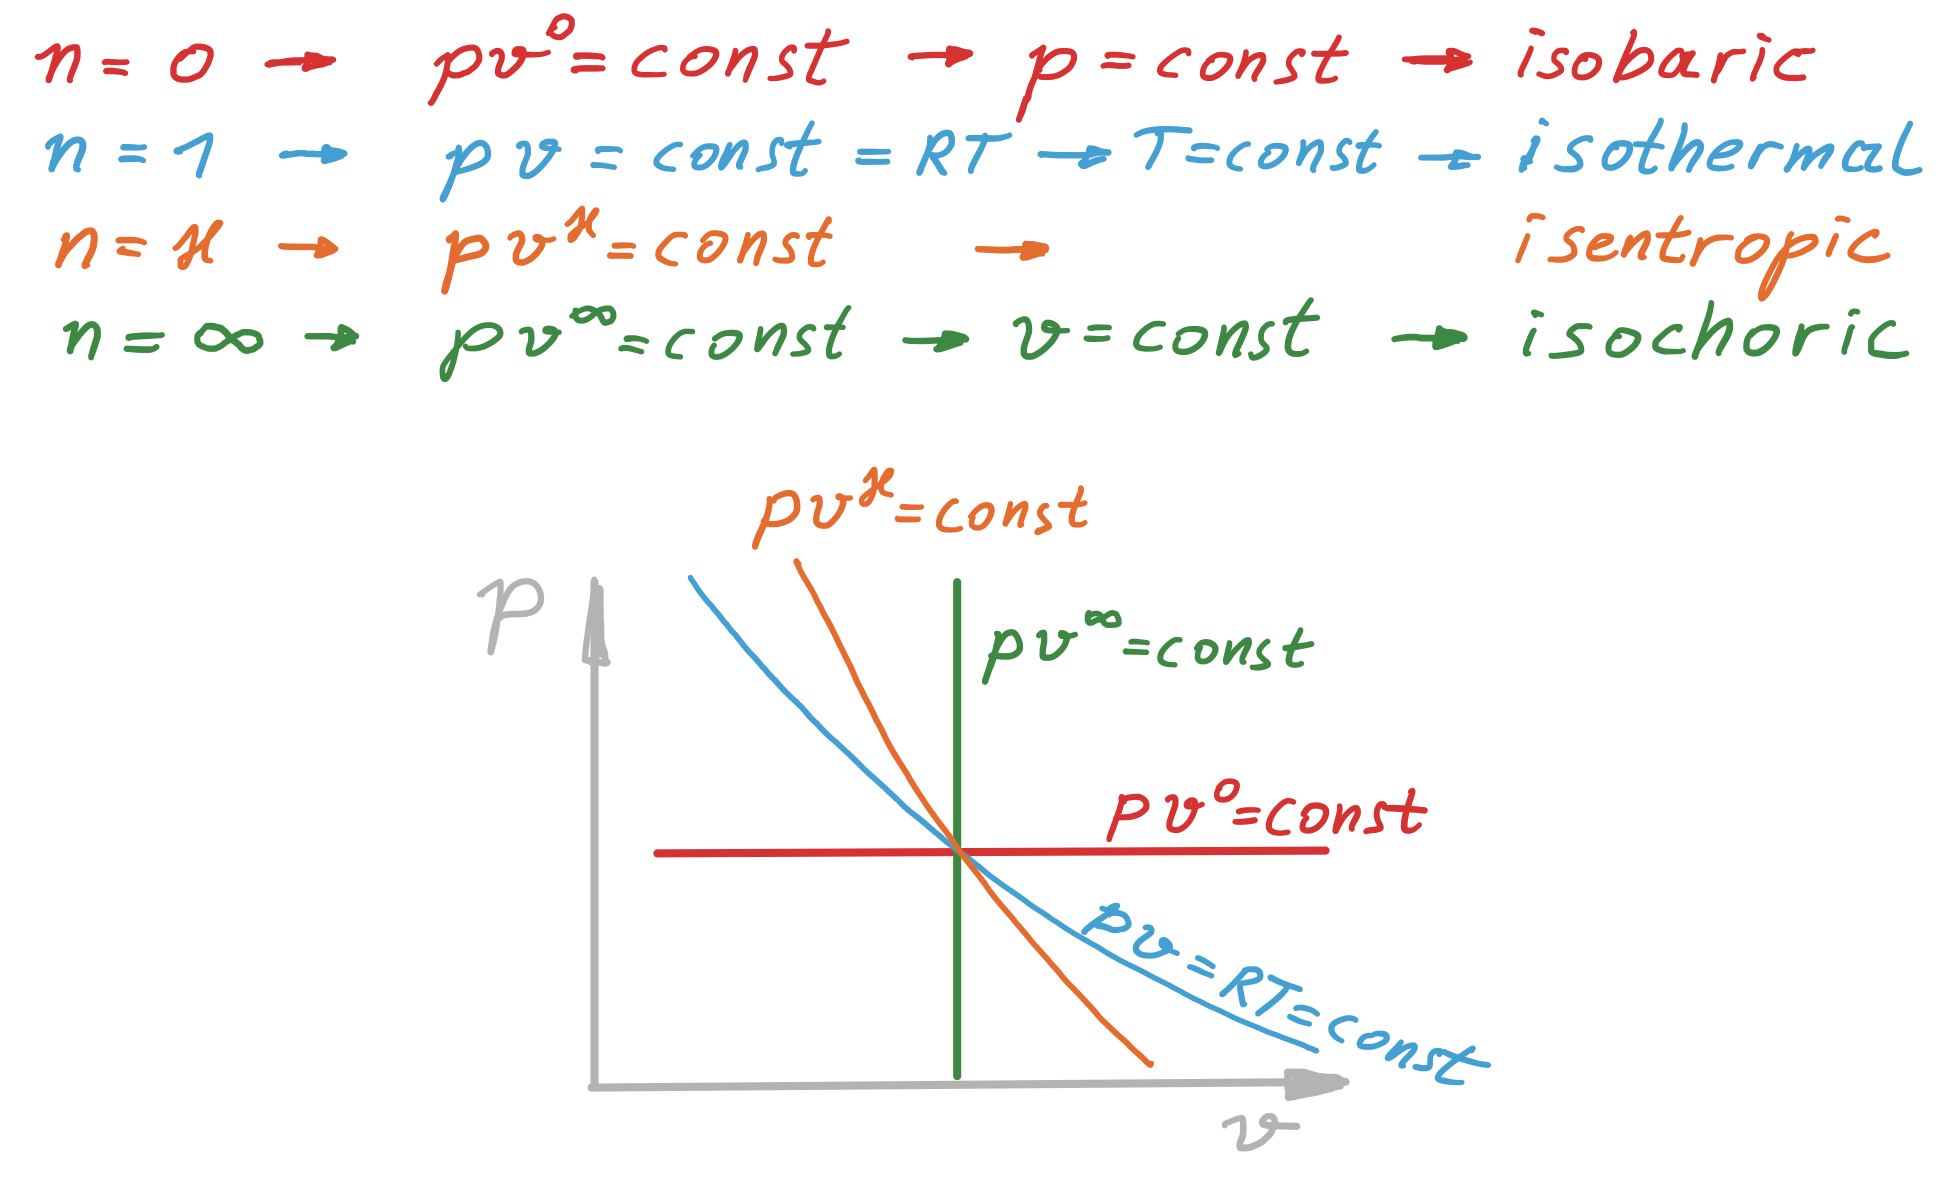
\includegraphics[width=100mm]{images/polytropic.png}}
  \caption{The graph for processes at different values of $n$.}
\end{figure}

\end{document}